\documentclass[11pt]{article}%
\usepackage[utf8]{inputenc}
\usepackage{todonotes}

\usepackage{amsfonts}
\usepackage{fancyhdr}
\usepackage{comment}
\usepackage[a4paper, top=2.5cm, bottom=2.5cm, left=2.2cm, right=2.2cm]%
{geometry}
\usepackage{times}
\usepackage{amsmath}
\usepackage{changepage}
\usepackage{amssymb}
\usepackage{graphicx}
\usepackage{float}
\usepackage{hyperref}
\usepackage{wrapfig}
\setcounter{MaxMatrixCols}{30}
\newenvironment{proof}[1][Proof]{\textbf{#1.} }{\ \rule{0.5em}{0.5em}}

\newcommand{\Q}{\mathbb{Q}}
\newcommand{\R}{\mathbb{R}}
\newcommand{\C}{\mathbb{C}}
\newcommand{\Z}{\mathbb{Z}}

\begin{document}

\title{Information Visualization : Mobility in Brussels}
\author{Bruno M. Cabral, Pierre Gerard, Titouan Christophe, Luiz N. Junior}
\date{Vrije Universiteit Brussel - May 2016}
\maketitle


\section{Introduction}

Brussels region public transportation is organized into a vast number of lines that are divided into metro, tramways and buses; so the system is quite susceptible to suffer with exceptional events that happen in the city, which many times cause delays on its lines schedules, consequently, affecting its users.


The main goal of the project is trying to answer two questions which are related to this context of mobility via information visualization:

\begin{enumerate}
	\item Is it possible to visualize the impact of street works or special events on brussels public transports?
	\item Are there areas in the city that are significantly less served by public transports?
\end{enumerate}

To this end, we built an interactive visualization that allows to explore the STIB network load and fluidity over time, compare it to the density of stops and put them in perspective with particular events happening in the city.

\begin{figure}[H]
    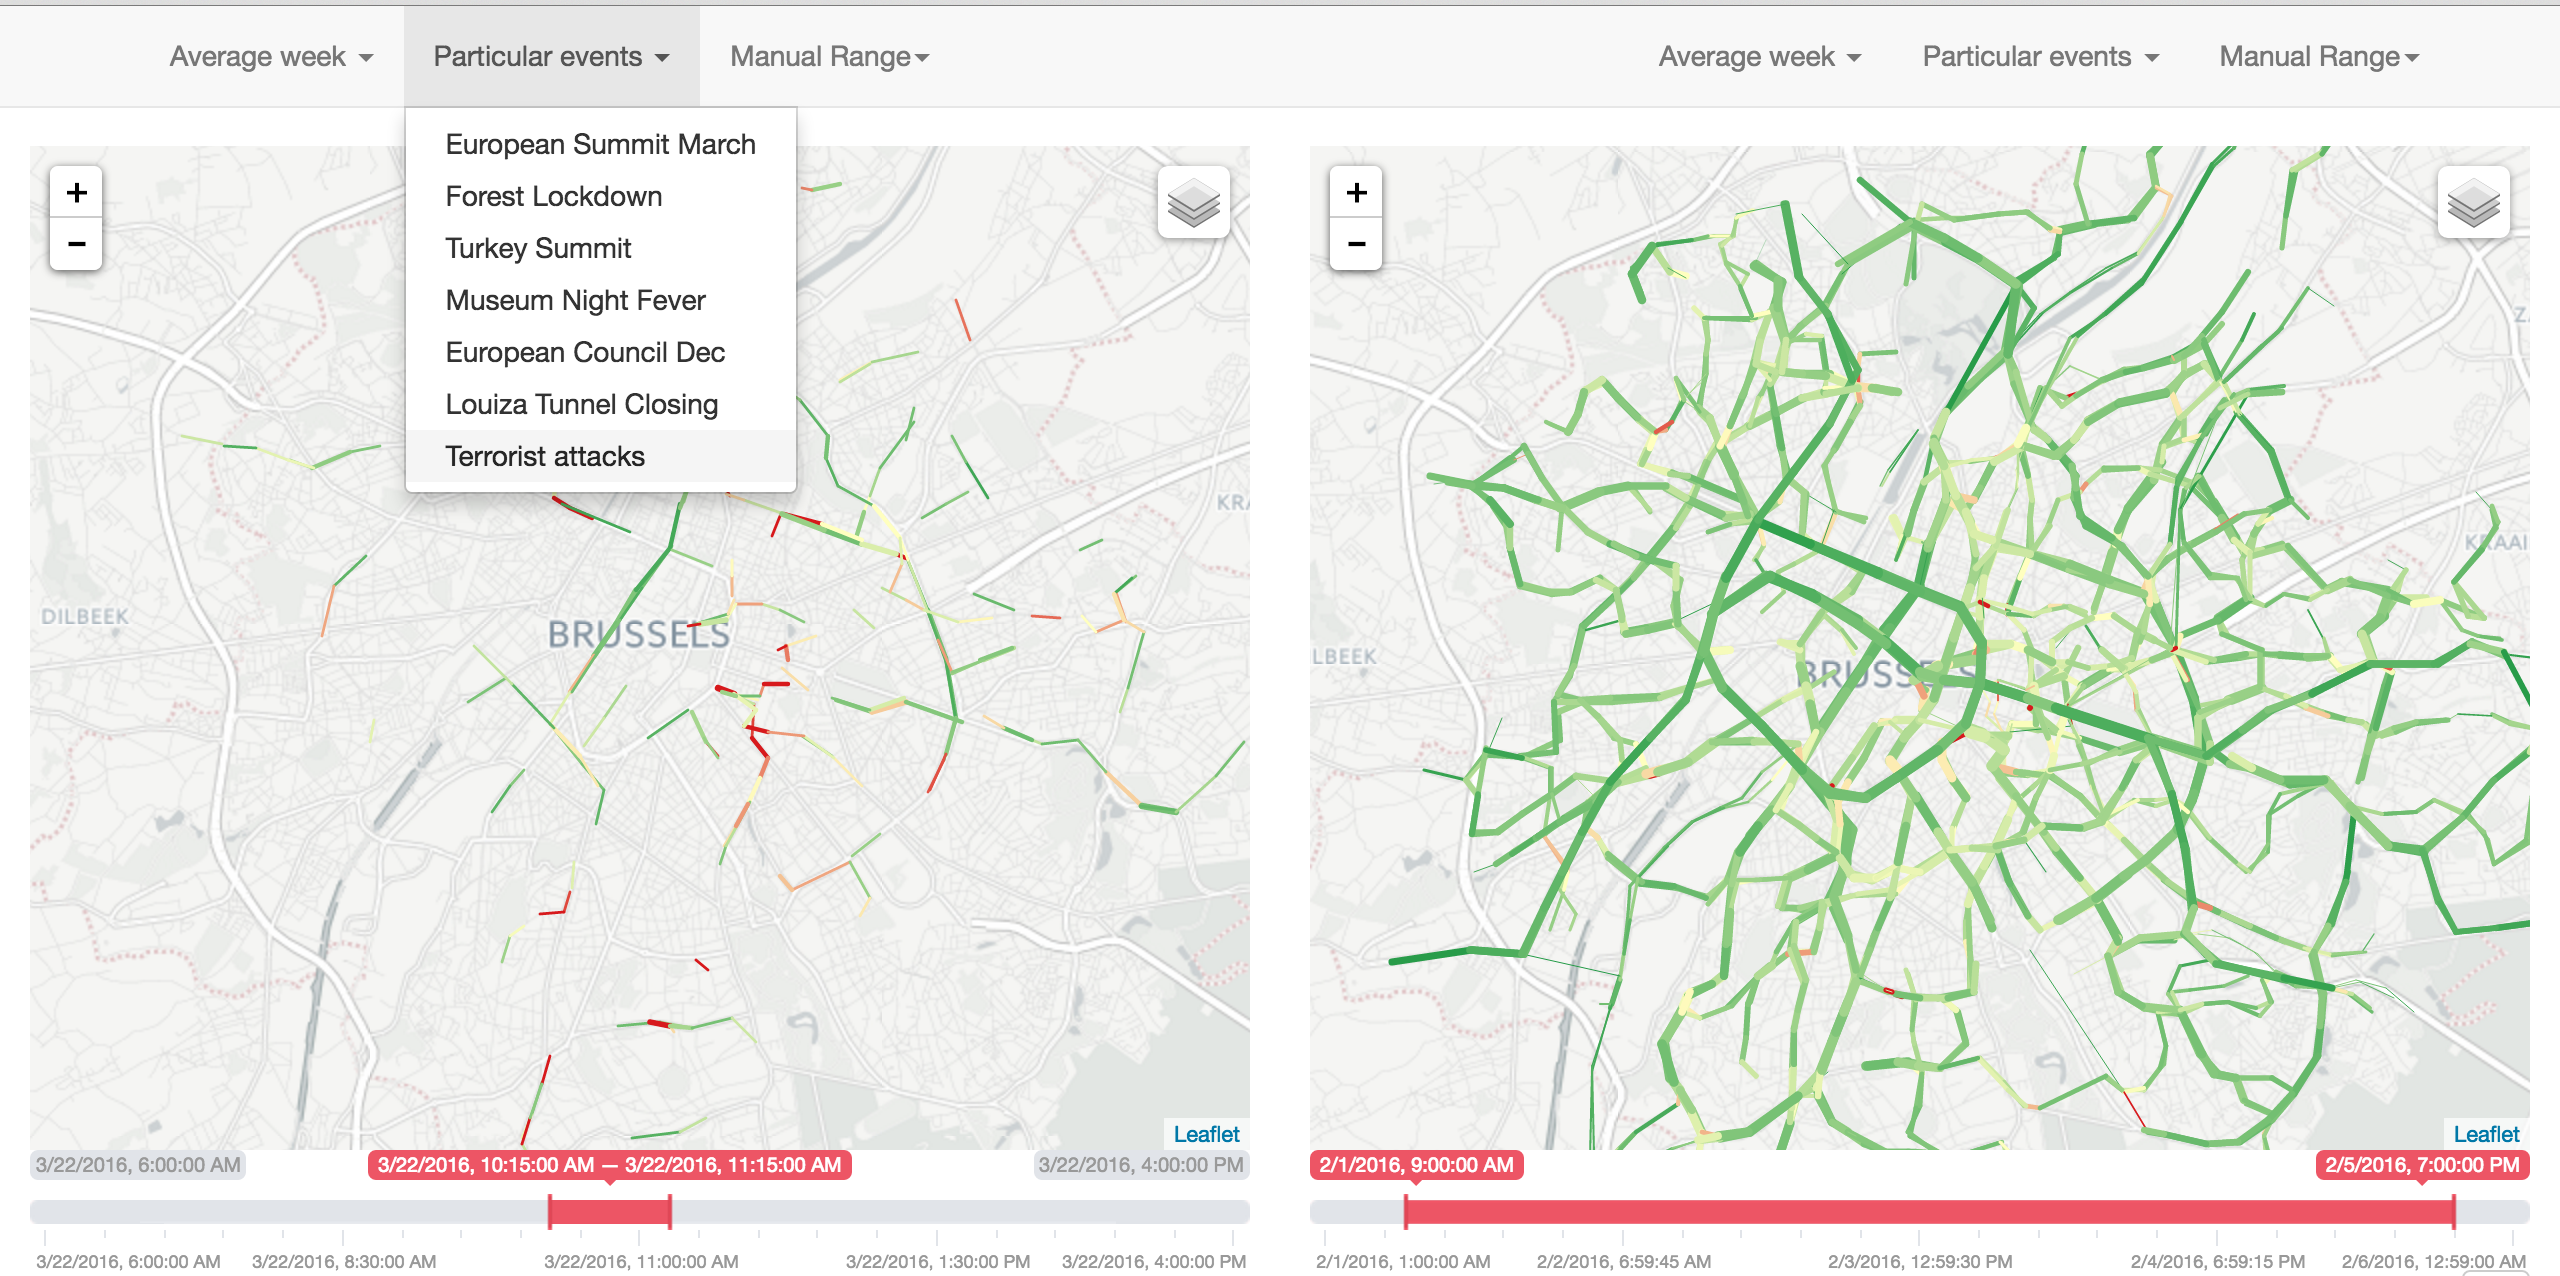
\includegraphics[width=\textwidth]{images/comparison.png}
    \caption{Overview of our visualization. The 2 maps allows for comparison between two differents time period. Each map also has a slider to precisely set the displayed time frame}
  \end{figure}

\section{Data sources}

\begin{minipage}{0.25\textwidth}
  \begin{figure}[H]
    \center
    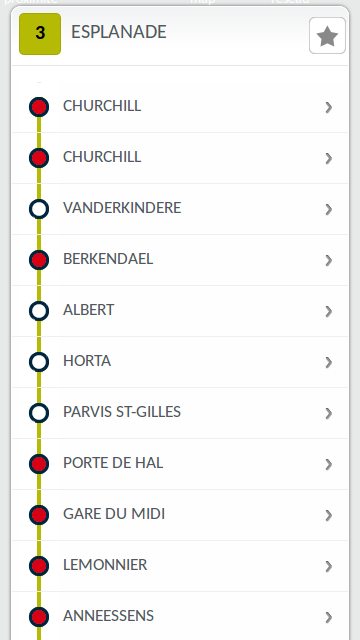
\includegraphics[width=\textwidth]{images/stibmobile.png}
    \caption{\href{http://m.stib.be/}{Mobile app}}
  \end{figure}
\end{minipage}\hfill
\begin{minipage}{0.7\textwidth}
  \subsection{Vehicles flow}
  In order to get the travel time for each line, a script is periodically querying the SITB mobile application API. We obtain a snapshot of the vehicles position every 20 seconds for each line. It is not possible to have a better resolution without trouble for the STIB servers. These snapshots are then processed to obtain the travel times. At this step, we have a set of tuples \texttt{(line, from\_stop\_id, to\_stop\_id, departure\_time, arrival\_time)}, stored in a relational database (PostgreSQL). As the amount of data is quite large, we rely on database indexes and aggregation functions, and http cache to make the application more fluid.

  \subsection{Lines Itineraries}
  It's worth noting that all the information related to the itineraries and colors of the lines were also collected from the STIB/MIVB real time website. For each line, we now:

  \begin{itemize}
      \item The itinerary, that is the sequence of stops a line pass by from a terminus to another
      \item The color of the line
      \item Wether it is a tramway, a metro or a bus line
  \end{itemize}
\end{minipage}

\subsection{Public Transportation Stops}
The public transportation network on Brussels region is managed by Brussels Intercommunal Transport Company (STIB/MIVB). The dataset providing all stops locations (coordinates) and names is available at Open Data Brussels web portal \footnote{\url{http://opendata.bruxelles.be/explore/dataset/arrets-stib/}}.

\subsection{Delay events}
In order to give a better perspective of how the transport system behaves under effect of extraordinary events, some specifics ones that happened in the city during the last months were added manually to the application, i.e. the european summit that happened in March of 2016.

Seeking to improve the system functionality, as soon as the user click on a predefined event, both maps are zoomed into the area where the aforementioned event took place. This takes in consideration the fact that an user may not know in which part of the city a certain happening occurred.
                       
\section{Architecture}
Our visualization is structured as a single page web application, written in ES6, and compiled into javascript using babeljs \footnote{\url{http://babeljs.io/}}. The project can be built using the command \texttt{npm run build} from the \texttt{app/} directory

We use Leaflet \footnote{\url{http://leafletjs.com/}} as map engine, the Ion Range Slider \footnote{\url{http://ionden.com/a/plugins/ion.rangeSlider/en.html}} for datetime pickers, and jQuery \footnote{\url{https://jquery.com/}} for DOM manipulation and asynchronous requests. We also use Bootstrap \footnote{\url{http://getbootstrap.com/}} for its reusable user interface components.

Access to the database is provided by an API written in Python with Flask \footnote{\url{http://flask.pocoo.org/}}

\section{The visualization}


\begin{minipage}{0.4\textwidth}
  \begin{figure}[H]
    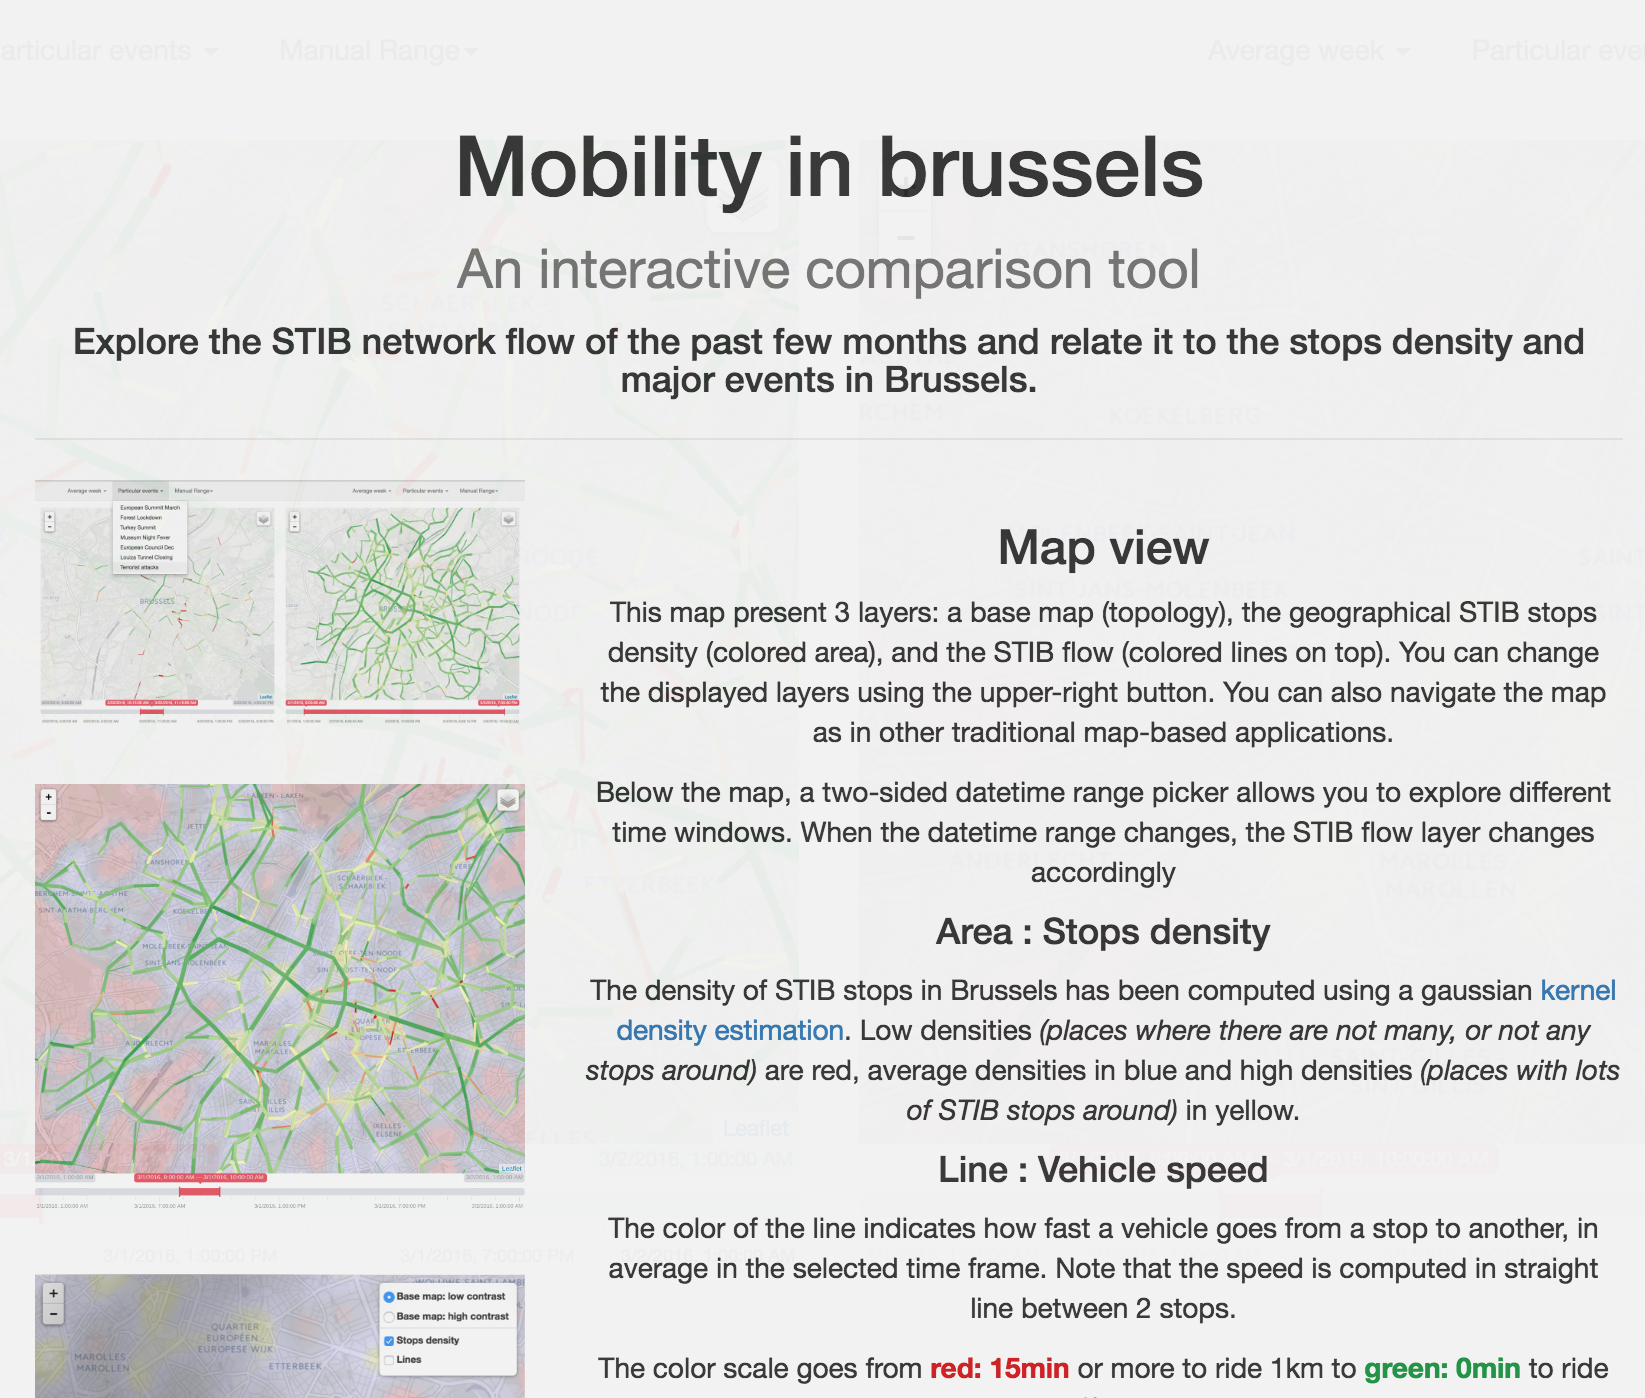
\includegraphics[width=\textwidth]{images/modal.png}
    \caption{Help modal}
  \end{figure}
\end{minipage}\hfill
\begin{minipage}{0.58\textwidth}
  \subsection{Modal}
  We created a modal to ease the way for unfamiliar users with our visualization. That is a documentation page overlaying the visualization itself providing guidance to the user. That idea come from other visualization found on the web (eg : World Atlas of Language Structures \cite{visuawithmodal}). The modal can be closed using the escape key or by clicking on a cross or a button.
\end{minipage}


\subsection{Map view}

This map present 3 layers: a base map (topology), the geographical STIB stops density (colored area), and the STIB flow (colored lines on top). The user can change the displayed layers using the upper-right button. You can also navigate the map as in other traditional map-based applications.

Below the map, a two-sided datetime range picker allows you to explore different time windows. When the datetime range changes, the STIB flow layer changes accordingly

\begin{minipage}{0.3\textwidth}
  \begin{figure}[H]
    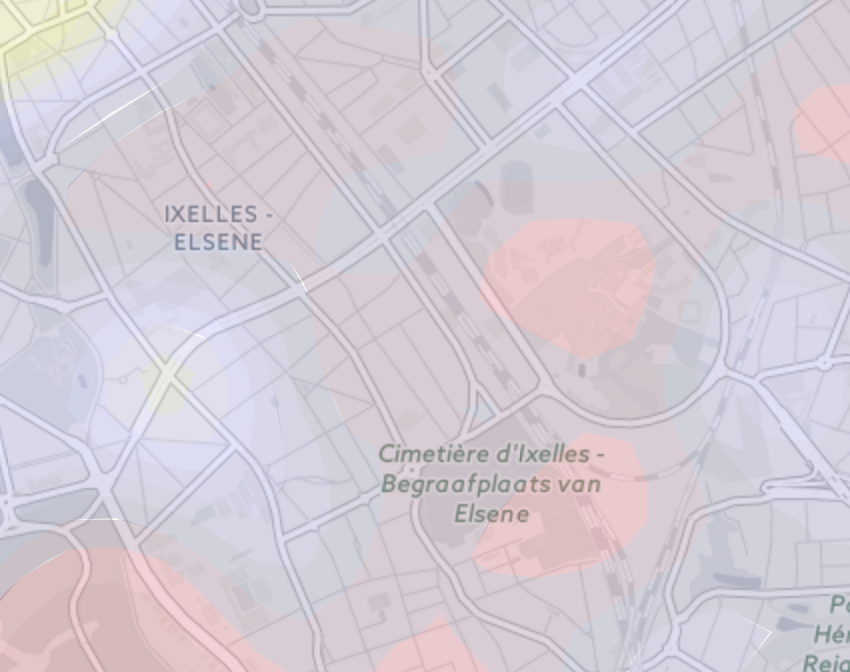
\includegraphics[width=\textwidth]{images/area.png}
    \caption{Stops density layer}
  \end{figure}
\end{minipage}\hfill
\begin{minipage}{0.6\textwidth}
  \subsubsection{Stop density}
  The density of STIB stops in Brussels has been computed using a gaussian kernel density estimation \cite{kdewiki}. Low densities (places where there are not many, or not any stops around) are red, average densities in blue and high densities (places with lots of STIB stops around) in yellow.
\end{minipage}

\begin{minipage}{0.3\textwidth}
  \begin{figure}[H]
    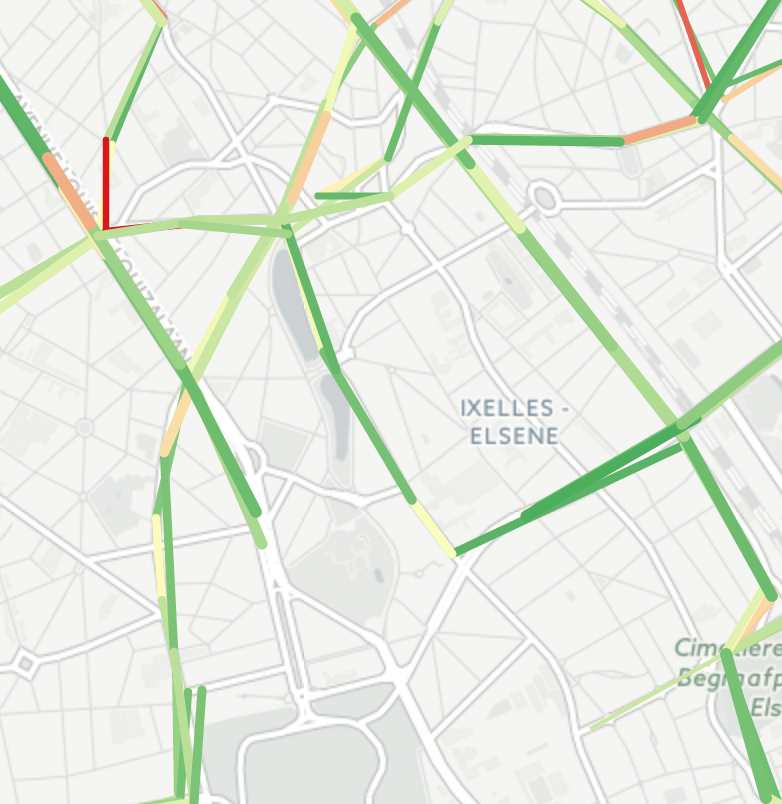
\includegraphics[width=\textwidth]{images/lines.png}
    \caption{STIB lines layer}
  \end{figure}
\end{minipage}\hfill
\begin{minipage}{0.6\textwidth}
  \subsubsection{Lines}
  The colour of the line indicates how fast a vehicle goes from a stop to another, in average in the selected time frame. Note that the speed is computed based on a straight line between 2 distinct stops.

  The colour scale goes from red to green, where red stands for a situation where a transport takes 15 minutes or more to travel 1 kilometer, and green represent a vehicle capable of traveling 1 kilometer in less than 60 seconds.

  Finally, the thickness of the lines indicates how many vehicles, per hour, in average passed by this section. An important remark is that this is valid for the selected time frame.
\end{minipage}

\begin{minipage}{0.3\textwidth}
  \begin{figure}[H]
    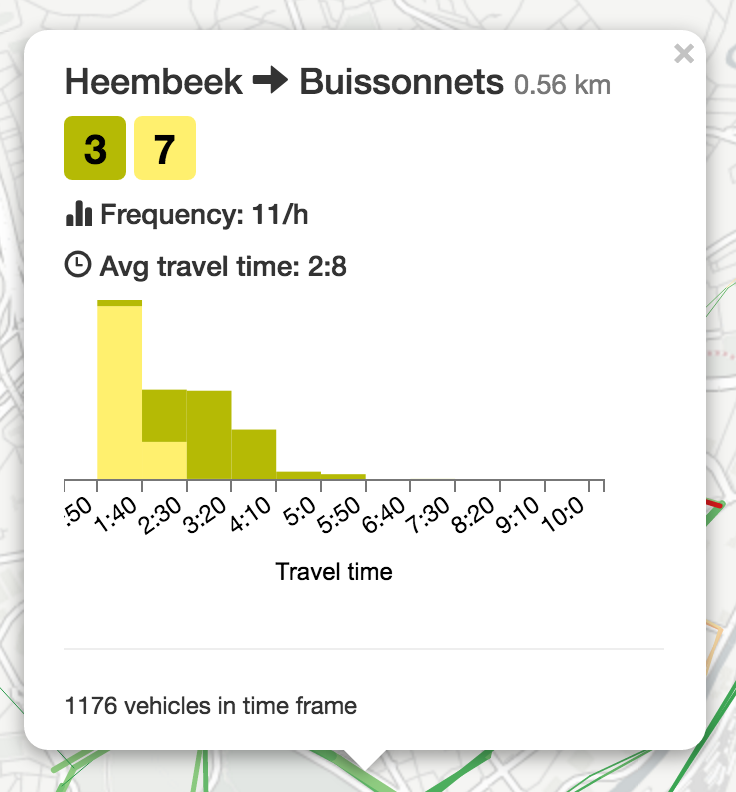
\includegraphics[width=\textwidth]{images/popup1.png}
    \caption{\label{fig:popup} The detailled tooltip}
  \end{figure}
\end{minipage}\hfill
\begin{minipage}{0.6\textwidth}
    \subsection{Detailed view}
    Clicking on a line open a tooltip offering detailed information about the line showing statistics about that line. The statistics include a D3 histogram of the traject time.
    \paragraph{Ah ha!} On Figure \ref{fig:popup}, we can clearly see that the 7 takes less time than the 3 on the traject from Heembeek to Buissonnets.
\end{minipage}

\begin{minipage}{0.3\textwidth}
  \begin{figure}[H]
    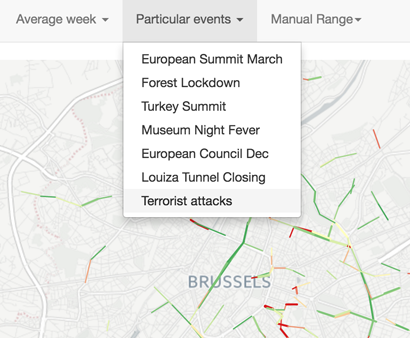
\includegraphics[width=\textwidth]{images/topbar.png}
    \caption{\label{fig:popup} The event chooser}
  \end{figure}
\end{minipage}\hfill
\begin{minipage}{0.6\textwidth}
  \subsection{Events and time selection}
  
  The navbar allows the user to choose a timeframe. The timeframe can be an average moment, a specific event or a precise moment in the time. The precise moment is selected trough a one sided slider.
\end{minipage}

\section{Acknowledgement}

We would like to thanks Nikita Marchant who provide us the delay data in the form of a postgresql relational database which he used for his bachelor thesis \cite{nikita}. 

\section{Conclusion}
We believe that our visualization help in the answering of the question which area is less deserved and the help in visualizing event that affect public transporation. 

 
\begin{thebibliography}{9}
 
\bibitem{nikita} 
Nikita Marchant: "Estimation en temps réel des temps de trajet dans un réseau de bus à l'aide de données historiques", 2016, \textit{bachelor thesis}
\\\url{https://github.com/C4ptainCrunch/info-f-308}

\bibitem{visuawithmodal} 
World Atlas of Language Structures,
\\\url{http://www.puffpuffproject.com/languages.html}

\bibitem{kdewiki} 
Kernel density estimation,
\\\url{https://en.wikipedia.org/wiki/Kernel_density_estimation}



\end{thebibliography}

\end{document}
